% ThermoTwin-3D --- progress presentation (Automation in Construction framing)
% Compile with:  pdflatex thermotwin_aic.tex   (run twice for the outline/refs)
% Uses only standard, universally-available packages (beamer, booktabs, tikz, amssymb).
\documentclass[aspectratio=169]{beamer}
\usetheme{Madrid}
\usecolortheme{whale}
\usepackage{booktabs}
\usepackage{amsmath,amssymb}
\usepackage{tikz}
\usepackage{xcolor}
\setbeamertemplate{navigation symbols}{}

% A small helper for the "win" tag used through the results section.
\newcommand{\win}[1]{{\color{green!55!black}\textbf{#1}}}
\newcommand{\unit}[1]{\,\mathrm{#1}}

\title[ThermoTwin-3D]{ThermoTwin-3D}
\subtitle{A geometry-resolved thermal twin of building envelopes from as-built scans}
\author{Y.\ Ansari}
\institute{Project progress review}
\date{\today}

\begin{document}

\begin{frame}[plain]
  \titlepage
  \begin{center}\small
    Forward prediction of the envelope thermal field \;$+$\; inverse recovery of
    U-values and thermal bridges from measured infrared.
  \end{center}
\end{frame}

\begin{frame}{Where we are going (one slide)}
  \begin{enumerate}
    \item \textbf{The problem} --- envelope heat loss and thermal bridges are invisible to today's tools.
    \item \textbf{The aim} --- a geometry-resolved thermal twin: scan $\to$ field $\to$ U-values and bridges.
    \item \textbf{The gap} --- nobody has joined the forward and inverse halves on real as-built geometry.
    \item \textbf{Data and metrics} --- what we trained and validated on, and how we score it.
    \item \textbf{Results} --- five findings, each a building block of the twin.
    \item \textbf{Contribution and next steps} --- toward an \emph{Automation in Construction} paper.
  \end{enumerate}
\end{frame}

% ---------------------------------------------------------------- problem
\begin{frame}{The problem: envelopes leak, and we cannot see where}
  \begin{itemize}
    \item Building \textbf{envelopes} (walls, roofs, junctions) drive a large share of heating and
          cooling demand. The biggest, least-understood losses are \textbf{thermal bridges} ---
          balcony slabs, concrete corners, steel studs that short-circuit the insulation.
    \item Today's practice sits at two extremes:
      \begin{itemize}
        \item \emph{Geometry-blind} --- the 1-D U-value calculation treats every wall as a flat slab;
              it cannot see a bridge.
        \item \emph{Qualitative} --- manual infrared (IR) walkthroughs show \emph{where} it is warm,
              but not \emph{how much} heat is lost or \emph{what} the U-value is.
      \end{itemize}
    \item Meanwhile, \textbf{as-built 3-D scans} (point clouds, CityGML, photogrammetry) are now routine
          on real projects. The opportunity: turn a scan into a \emph{quantitative} thermal model.
  \end{itemize}
\end{frame}

% ---------------------------------------------------------------- aim
\begin{frame}{What we aim to build: a thermal twin with two directions}
  \begin{columns}[T]
    \begin{column}{0.5\textwidth}
      \textbf{Forward (prediction)}\\[2pt]
      Feed real envelope geometry $+$ materials $\Rightarrow$ predict the temperature / heat-flux
      \textbf{field} $\theta$ over the whole surface --- in milliseconds, not the seconds-to-minutes
      of a finite-element solve.
    \end{column}
    \begin{column}{0.5\textwidth}
      \textbf{Inverse (diagnosis)}\\[2pt]
      Feed a \textbf{measured IR field} $\Rightarrow$ recover \textbf{per-surface U-values} and
      \textbf{localized thermal-bridge conductances}, with a \textbf{calibrated uncertainty} on every
      estimate.
    \end{column}
  \end{columns}
  \vspace{0.6em}
  \begin{block}{In one sentence}
    A digital twin that reads a building's thermal behaviour off its as-built geometry --- and reads
    its hidden defects back out of a thermal image.
  \end{block}
\end{frame}

% ---------------------------------------------------------------- why
\begin{frame}{Why it matters for construction automation}
  \begin{itemize}
    \item \textbf{Retrofit at scale.} Automatically rank where a building loses heat, and target
          insulation / repair where it pays off --- per surface, per bridge.
    \item \textbf{Quantitative, not qualitative.} Turns an IR survey from ``looks warm here'' into
          ``this junction is $\Psi = \dots$, with this confidence.''
    \item \textbf{Geometry-aware, not lumped.} Works on the real, irregular as-built shell, not an
          idealized box --- which is exactly where bridges live.
    \item \textbf{Fast enough to be interactive.} A twin you can re-query for what-if retrofit
          scenarios, or run city-wide.
  \end{itemize}
\end{frame}

% ---------------------------------------------------------------- gap
\begin{frame}{The research gap}
  Two mature but \textbf{separate} research streams:
  \begin{itemize}
    \item \textbf{Forward stream} --- geometry-conditioned neural operators that predict physical
          fields on complex geometry (fast surrogates for simulation).
    \item \textbf{Inverse stream} --- inverse thermography that recovers material properties
          (U-values, $\Psi$) from surface temperature.
  \end{itemize}
  \vspace{0.4em}
  \begin{alertblock}{The gap}
    Neither stream has been joined \emph{on real as-built 3-D building envelopes}. There is no
    end-to-end, geometry-resolved neural thermal twin that goes scan $\to$ field $\to$ inverse
    U/bridge recovery. \textbf{Closing that loop is our contribution.}
  \end{alertblock}
\end{frame}

% ---------------------------------------------------------------- approach / pipeline
\begin{frame}{The approach: one pipeline, end to end}
  \begin{center}
  \scalebox{0.92}{
  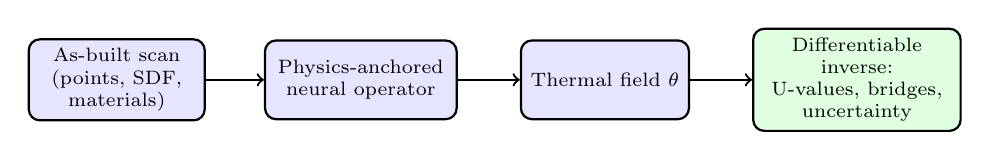
\begin{tikzpicture}[every node/.style={draw, rounded corners, align=center,
       font=\scriptsize, minimum height=1.0cm}, thick]
    \node (a) at (0,0)   [fill=blue!10,  text width=2.0cm] {As-built scan\\(points, SDF, materials)};
    \node (b) at (3.1,0) [fill=blue!10,  text width=2.2cm] {Physics-anchored neural operator};
    \node (c) at (6.2,0) [fill=blue!10,  text width=1.9cm] {Thermal field $\theta$};
    \node (d) at (9.4,0) [fill=green!12, text width=2.4cm] {Differentiable inverse:\\U-values, bridges, uncertainty};
    \draw[->] (a)--(b);  \draw[->] (b)--(c);  \draw[->] (c)--(d);
  \end{tikzpicture}}
  \end{center}
  \vspace{0.3em}
  \begin{itemize}\small
    \item The \textbf{forward operator} is anchored on a cheap analytic \emph{physics prior} (the 1-D
          conduction field) and learns only the \emph{correction} the prior misses --- this is the key
          that makes it work on real geometry (Result~1).
    \item The \textbf{inverse} runs that differentiable forward backwards: it searches for the
          properties that best explain a measured field, regularized and uncertainty-aware.
  \end{itemize}
\end{frame}

% ---------------------------------------------------------------- datasets
\begin{frame}{Datasets: synthetic, real geometry, and measured reality}
  \footnotesize
  \begin{tabular}{@{}lll@{}}
    \toprule
    \textbf{Role} & \textbf{Dataset} & \textbf{What it gives} \\
    \midrule
    Geometry $+$ physics GT & Synthetic (box / irregular / hard) & controlled bridges, known answer \\
                            & Real-CityGML LoD2 \& LoD3 (TUM2TWIN) & 27 real building shells, 2 fidelities \\
                            & 3D-BAG (Amsterdam) & $\sim$160 real urban shells \\
                            & DOE Reference Buildings & real construction libraries \\
    \midrule
    Measured validation     & Twin Houses & in-situ measured U-values \\
                            & ThermoScenes & calibrated ${}^{\circ}$C facade thermal fields \\
                            & TUM2TWIN-TIR & airborne infrared orthophoto \\
                            & Dublin (ISO-9869) & measured heat-flux + U-values \\
    \midrule
    Cross-domain benchmark  & Conduction-with-inclusions (WHNO / EIT) & published, sharp-contrast fields \\
    \bottomrule
  \end{tabular}
  \vspace{0.5em}
  \begin{itemize}\small
    \item Direct corpora carry \emph{simulated} ground-truth fields; the measured datasets are the
          independent reality check.
  \end{itemize}
\end{frame}

% ---------------------------------------------------------------- metrics
\begin{frame}{Metrics: we always pair an ML metric with a building metric}
  \begin{itemize}
    \item \textbf{Field accuracy} --- relative-$L_2$ error of the predicted field; physical RMSE in
          kelvin.
    \item \textbf{Building-relevant} --- per-surface \textbf{U-value error} (MAE, W/m$^2$K); thermal-bridge
          \textbf{localization} (precision / recall / IoU).
    \item \textbf{Bridge-focused} --- ``correction relative-$L_2$'', normalized so the \emph{analytic
          prior} scores exactly $1.0$. A value $<1$ means the learned operator \emph{genuinely beats
          physics-you-already-knew} at the bridges.
    \item \textbf{Uncertainty} --- calibration: does the predicted confidence interval actually cover
          the truth (ideal $1\sigma$ coverage $\approx 0.68$)?
    \item \textbf{Efficiency} --- speedup versus a finite-volume solve.
  \end{itemize}
\end{frame}

% ============================================================ RESULTS
\section{Results}

\begin{frame}{Five results --- each a building block of the twin}
  \begin{enumerate}
    \item \win{The physics-residual recipe} makes geometry operators \emph{work} on real scans.
    \item \win{A comprehensive benchmark} maps exactly \emph{where} learning adds value.
    \item \win{The inverse twin} reads thermal bridges and U-values back out of the field.
    \item \win{Calibrated uncertainty} makes every estimate trustworthy.
    \item \win{Measured-data validation} corroborates the whole chain.
  \end{enumerate}
\end{frame}

% ---------------------------------------------------------------- result 1
\begin{frame}{Result 1 --- the physics-residual recipe is the enabler}
  \textbf{Finding.} A neural operator on its own \emph{fails} on real scanned geometry. Anchor it on the
  analytic physics prior --- have it predict only the \emph{correction} --- and it becomes accurate,
  \emph{across every architecture we tried}.
  \vspace{0.4em}
  \begin{center}\small
  \begin{tabular}{@{}lcc@{}}
    \toprule
    Backbone (on real-CityGML) & data-only field rel-$L_2$ & \textbf{$+$ physics-residual} \\
    \midrule
    Transolver (transformer)   & 0.245 & \textbf{0.018} \\
    GINO (graph operator)      & 0.808 & \textbf{0.025} \\
    PointNet++ (point network) & 0.224 & \textbf{0.015} \\
    DeepONet (branch/trunk)    & 0.461 & \textbf{0.016} \\
    \bottomrule
  \end{tabular}
  \end{center}
  \vspace{0.3em}
  \begin{itemize}\small
    \item Lower is better; $10\times$--$50\times$ improvement, from \emph{unusable} to \emph{accurate}.
    \item \win{Take-away:} on real as-built geometry, a physics-residual recipe is \emph{necessary} ---
          and it is \emph{architecture-agnostic}. This is a clean, general result.
  \end{itemize}
\end{frame}

% ---------------------------------------------------------------- result 2
\begin{frame}{Result 2 --- where does learning actually pay off?}
  We benchmarked \textbf{14 models} across \textbf{7 corpora} and \textbf{9 metrics} --- the most
  thorough comparison we could build --- to answer one question: \emph{when is the neural operator
  worth it over the cheap physics prior?}
  \vspace{0.4em}
  \begin{center}\small
  \begin{tabular}{@{}lcc@{}}
    \toprule
    Regime & bridge correction rel-$L_2$ & operator gain over prior \\
    \midrule
    Severe bridges (synthetic ``hard'')      & 0.36 & \win{$\sim$64\% better} \\
    Real clear-wall envelopes (CityGML)       & 0.88--0.92 & $\sim$10\% better \\
    Near-ideal walls (DOE)                    & $\approx 1.0$ & prior already optimal \\
    \bottomrule
  \end{tabular}
  \end{center}
  \vspace{0.3em}
  \begin{itemize}\small
    \item \win{The map:} the physics prior handles the smooth bulk near-perfectly; the operator earns
          its keep \emph{in proportion to thermal-bridge severity}.
    \item \win{Practical rule:} use the prior for the wall, the operator for the bridges --- and this is
          exactly what motivates the \emph{inverse}, where the bridges are the whole point.
  \end{itemize}
\end{frame}

% ---------------------------------------------------------------- result 3
\begin{frame}{Result 3 --- the inverse twin reads bridges and U back out}
  Given a thermal field, recover the conductivity / bridge map and the per-surface U-value.
  \vspace{0.3em}
  \begin{center}\small
  \begin{tabular}{@{}lccc@{}}
    \toprule
    Recovery target & severe (``hard'') & real-CityGML & LoD3 \\
    \midrule
    Thermal-bridge localization (IoU)        & \textbf{0.51} & 0.42 & 0.32 \\
    \quad precision / recall                 & 0.57 / 0.74 & \textbf{0.92} / 0.44 & \textbf{0.88} / 0.33 \\
    Per-surface U-MAE (W/m$^2$K)             & $\sim$0.04 & 0.001--0.002 & 0.002 \\
    \bottomrule
  \end{tabular}
  \end{center}
  \vspace{0.3em}
  \begin{itemize}\small
    \item \win{Bridges are recovered} --- high IoU where they are strong, and \emph{high precision}
          on real geometry (when the twin flags a bridge, it is right).
    \item \win{We resolve an inherent ill-posedness.} Naive optimization fits the field but recovers
          the \emph{wrong} properties (the inverse is non-unique). A \emph{learned} inverse recovers the
          true structure --- a genuine methodological finding.
    \item U-values are recovered accurately; on real walls U is near clear-wall, so the inverse's real
          content is the bridges.
  \end{itemize}
\end{frame}

% ---------------------------------------------------------------- result 4
\begin{frame}{Result 4 --- the twin knows when to trust itself}
  An estimate without uncertainty is not actionable for an engineer. We add a learned
  \textbf{uncertainty head} that predicts a confidence on every point.
  \vspace{0.3em}
  \begin{center}\small
  \begin{tabular}{@{}lcc@{}}
    \toprule
    & $1\sigma$ coverage (ideal $\approx 0.68$) & error--uncertainty correlation \\
    \midrule
    Learned uncertainty head (synthetic) & \textbf{0.69--0.72} & \textbf{0.64--0.80} \\
    Learned uncertainty head (real geom.) & 0.92--0.97 (conservative) & 0.44--0.63 \\
    \midrule
    Naive ensemble uncertainty (baseline) & 0.18--0.36 (badly off) & 0.07--0.30 \\
    \bottomrule
  \end{tabular}
  \end{center}
  \vspace{0.3em}
  \begin{itemize}\small
    \item \win{Well-calibrated} on synthetic geometry (coverage matches the ideal), conservative but
          coherent on real geometry --- and it \emph{far} outperforms the naive baseline.
    \item Bonus: the uncertainty map doubles as a \emph{bridge-reliability indicator} --- it lights up
          exactly where the prior is least trustworthy.
  \end{itemize}
\end{frame}

% ---------------------------------------------------------------- result 5
\begin{frame}{Result 5 --- validation against measured reality}
  The chain above is trained on simulated fields; these are the independent, \emph{measured} checks.
  \begin{itemize}
    \item \textbf{Twin Houses} (in-situ U-values): per-element \win{U-MAE $= 0.004\unit{W/m^2K}$},
          8 of 9 elements exact --- the one miss is a roof rafter, a real bridge the 1-D prior cannot see.
    \item \textbf{ThermoScenes} (calibrated ${}^{\circ}$C facade field): a geometry-local model explains
          \win{$\sim$63\%} of the measured field; the localized residual ($\sigma \approx 0.66\unit{K}$)
          \emph{is} the thermal-bridge signal --- precisely the inverse target.
    \item \textbf{TUM2TWIN-TIR} (airborne IR): measured heat-loss anomalies land \win{$2.1\times$} more
          on the modelled envelopes than off them.
  \end{itemize}
  \vspace{0.3em}
  \begin{block}{Plus: speed}
    The twin predicts a field in \win{$\sim$2 ms} versus a finite-volume solve of seconds to
    $\sim$30\,s --- up to $\sim$$10^{4}\times$ faster. City-scale and interactive use become possible.
  \end{block}
\end{frame}

% ---------------------------------------------------------------- contribution
\begin{frame}{Contribution and novelty}
  \begin{block}{The contribution is the \emph{system}}
    The first \textbf{end-to-end, geometry-resolved neural thermal twin of building envelopes}:
    \;scan $\to$ thermal field $\to$ inverse recovery of per-surface U-values and thermal bridges,
    with calibrated uncertainty --- on \emph{real as-built} geometry.
  \end{block}
  \vspace{0.2em}
  Within it, three findings stand on their own:
  \begin{enumerate}\small
    \item A \textbf{physics-residual recipe} is necessary --- and architecture-agnostic --- for neural
          operators on real scanned geometry.
    \item Learned operators add value \textbf{in proportion to thermal-bridge severity}; the physics prior
          is the right workhorse for the bulk.
    \item A \textbf{learned inverse resolves the ill-posedness} of property recovery that pure optimization
          cannot --- with \emph{calibrated} uncertainty.
  \end{enumerate}
  \vspace{0.2em}
  \centerline{\textbf{Target venue: \emph{Automation in Construction}} --- a construction-automation contribution, not an ML-mechanism one.}
\end{frame}

% ---------------------------------------------------------------- limitations / next
\begin{frame}{Honest limitations and next steps}
  \begin{itemize}
    \item \textbf{Ground-truth credibility.} Our bridge fields are simulated; the next step is validating
          them against an independent solver and the ISO-10211 thermal-bridge benchmark cases.
    \item \textbf{Measured-field inverse.} We validate \emph{U-values} on measured data today; running the
          inverse on a fully measured 3-D thermal field is the headline experiment to close.
    \item \textbf{Identifiability.} Surface IR under-determines interior properties; U-values and
          $\Psi$ (integrated quantities) are what is recoverable, and our uncertainty honestly reflects the rest.
  \end{itemize}
  \vspace{0.3em}
  \begin{block}{Roadmap to the paper}
    Credible bridge GT $\to$ measured-field inverse $\to$ retrofit what-if demonstration
    $\to$ \emph{Automation in Construction} submission.
  \end{block}
\end{frame}

% ---------------------------------------------------------------- conclusion
\begin{frame}{In summary}
  \begin{itemize}
    \item We set out to turn an \textbf{as-built scan} into a \textbf{quantitative thermal twin} of a
          building envelope.
    \item We showed a \textbf{physics-residual recipe} makes neural operators work on real geometry,
          \textbf{mapped} where learning pays off, built an \textbf{inverse} that recovers thermal
          bridges and U-values, made it \textbf{uncertainty-aware}, and \textbf{validated} against
          measured data.
    \item The result is the \textbf{first end-to-end geometry-resolved thermal twin} of building
          envelopes --- the contribution we take to \emph{Automation in Construction}.
  \end{itemize}
  \vspace{0.6em}
  \centerline{\large Thank you --- questions welcome.}
\end{frame}

\end{document}
